In a gesture to plot the power profile, propose the optimal riding strategy and test the sensitivity of the model, several works are done to build it and then solve the problem.
\begin{itemize}
	\item{\bf Accessing the data}. As it's hard to get real-time speed data of a certain athlete in a formal competition, we changed our course to excavate data from standard pace, past papers and other resources.The data sources are summarized in table [\ref{data}].
		\begin{table}[htbp]
				%	\renewcommand\arraystretch{1.3}
		%	\setlength\tabcolsep{13pt}%调列距
			\setlength{\belowcaptionskip}{0.2cm}
		\centering
		\caption{Data Source Collection}
		\begin{tabular}{cc}
			\toprule[2pt]
			Dataset & Website Source \\
			\midrule
			Cycling power charts & \textcolor[rgb]{ .02,  .388,  .757}{https://www.trainingpeaks.com/blog/power-profiling/} \\
			UCI results & \textcolor[rgb]{ .02,  .388,  .757}{https://www.flanders2021.com/en/races} \\
			Olympics results & \textcolor[rgb]{ .02,  .388,  .757}{https://www.procyclingstats.com/race/olympic-games-itt/2021/result} \\
			Maps  & \textcolor[rgb]{ .02,  .388,  .757}{https://www.openstreetmap.org/about/} \\
			Cycling details & \textcolor[rgb]{ .02,  .388,  .757}{https://www.strava.com/activities} \\
			\bottomrule[2pt]
		\end{tabular}%
		\label{data}%
	\end{table}%
	\item {\bf Presenting our model}. In order to investigate the problem deeper, we divide our model into three sub-models. The first one is the establishment of \emph{Power Curve Fitting} to describe athletes' ability in different exercise intensity. The second one is about power distribution during competition process, \emph{Power-Time-Energy Equation}, which establishes the relationship between output energy and demand energy. The third one is to solve the optimal strategy for a certain player and certain competition.
	
	% TODO: \usepackage{graphicx} required
	\begin{figure}
		\centering
		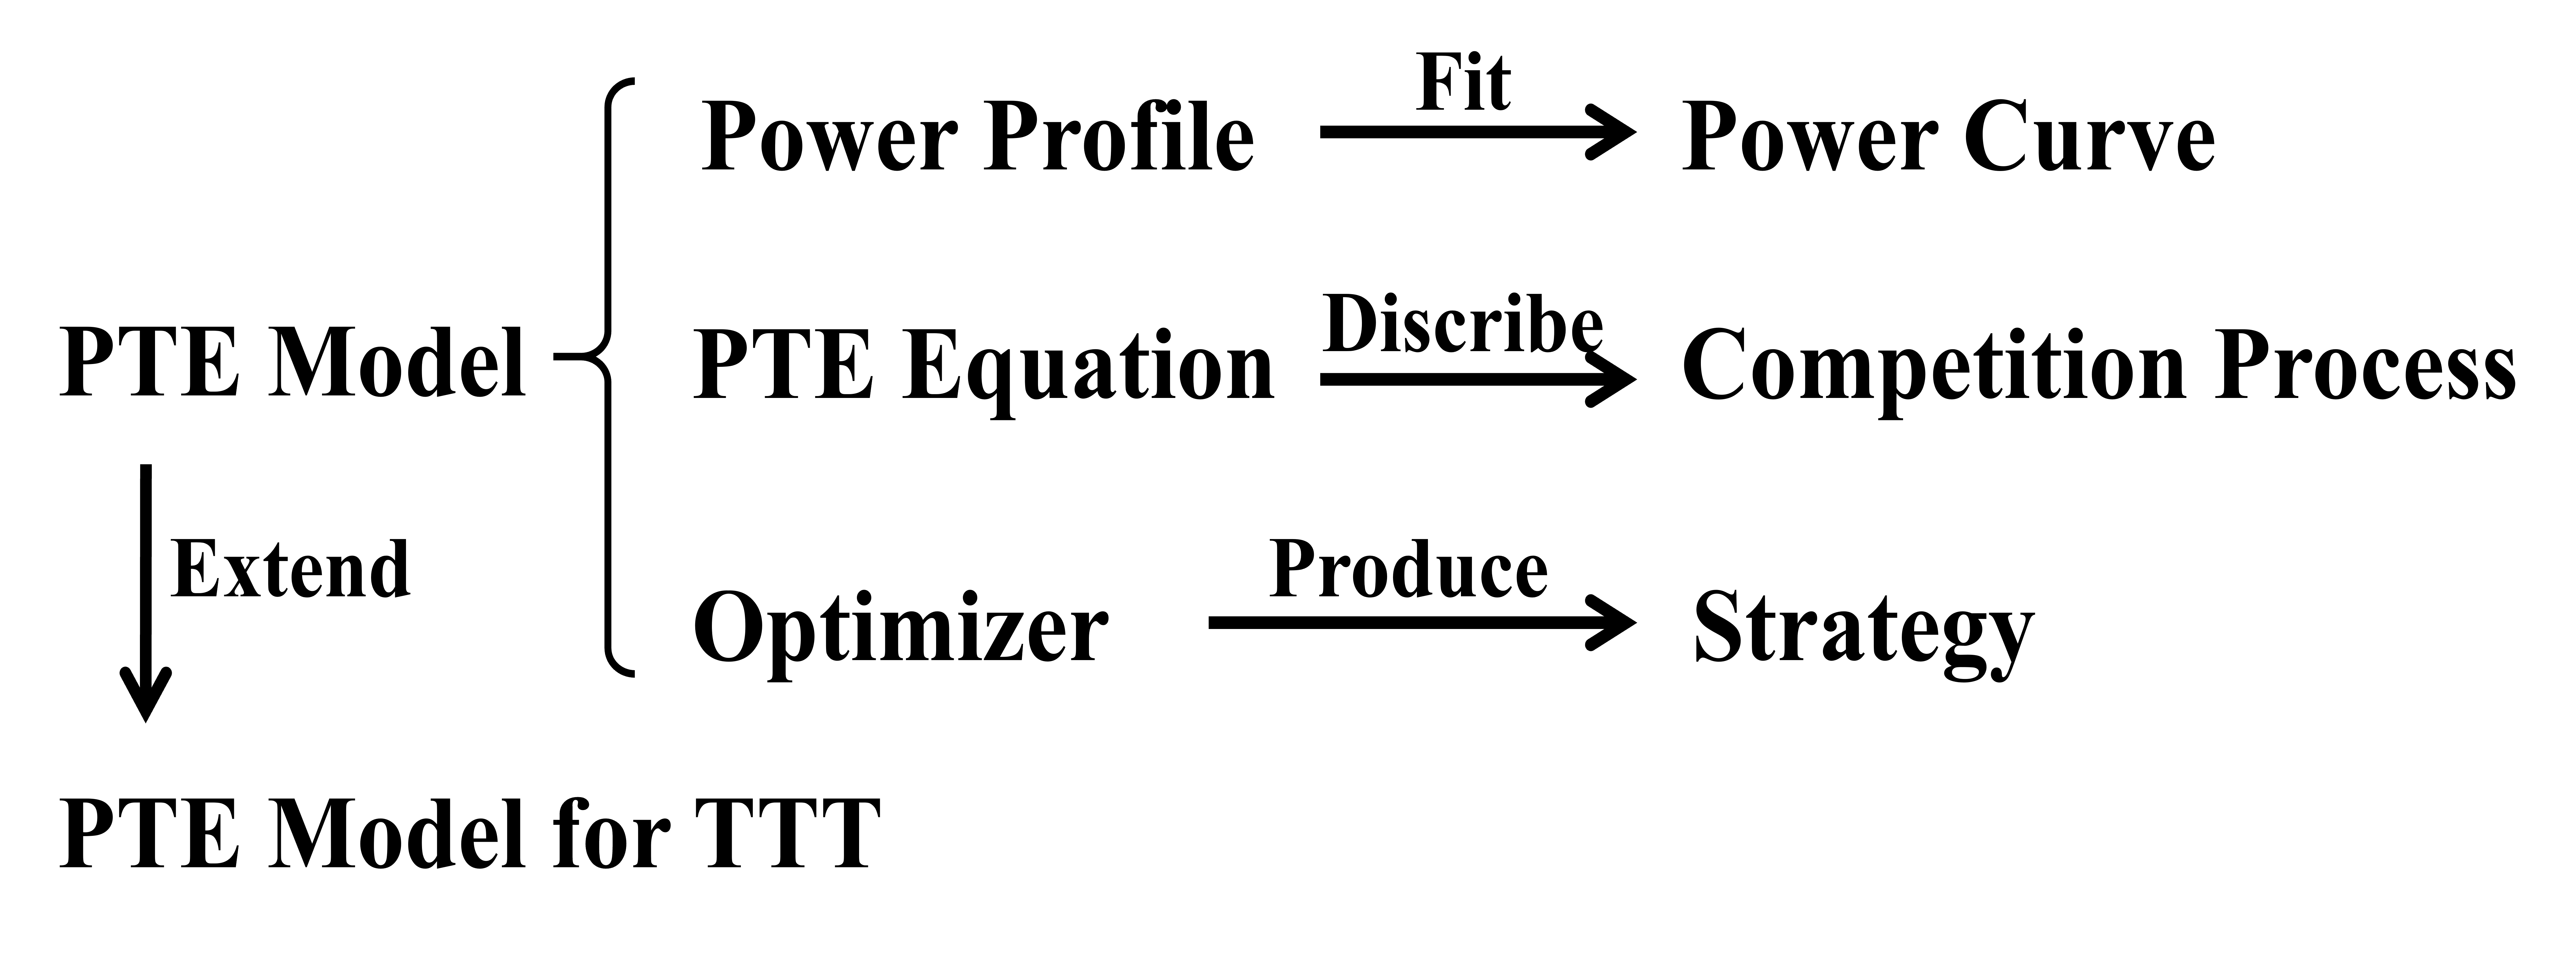
\includegraphics[width=0.7\linewidth]{image/liucheng}
		\caption{Structure chart}
		\label{liucheng}
	\end{figure}
	
	\item {\bf Sensitivity analysis and extension}.Taking weather condition and rider deviations into account, we apply extended model with UCI data to evaluate the reliability of our model through sensitivity analysis. Also, we extend our model to team time trial. 
	
\end{itemize}
